\chapter{Аналитический раздел}
В данном разделе будут рассмотрены теоретически основы работы алгоритмов полного перебора и муравьиного алгоритма для задачи коммивояжера.

\section{Описание задачи коммивояжера}
Задача коммивояжера может быть описана следующим образом - существует некоторе количество городов, каждый из которых связан с другими путями, имеющими определённую длину. Необходимо найти самый выгодный путь, начинающийся в исходном городе и проходящий ровно один раз через каждый из городов с последующим возвратом в исходный город.

Для представления задачи мы будем использовать графовую модель. Город представляется как один из узлов графа, а пути к другим городам - как рёбра. Критерий выгодности представляется как метка на ребре, обозначающая расстояние между городами, которые это ребро соединяет. Модельный граф задачи является полностью связным, то есть между любой произвольной парой различных вершин существует ребро с ненулевой меткой.

\section{Алгоритм полного перебора}
Пусть существует N городов, представленных в виде графовой модели. Для решения задачи коммивояджера методом полного перебора, нам необходимо перебрать всевозможные корректные для этой задачи пути. Данный метод даёт гарантированно идеальное решение для любого графа, однако сложность этого алгоритма не позволяет применять его для реальных задач, поскольку в следствие его рекурсивности сложность его составляет M!, что приводит к экспоненциальному росту времени выполнения программы в зависимости от количества городов.

\section{Муравьиный алгоритм}
В практических ситуациях идеальностью решения можно принебречь, если полученное решение является достаточно приближенным к нему, чтобы удовлетворять практическим запросам. Методы, которые работают, опираясь на это условие, называются эвримтическими, и решают задачу за гораздо более меньшее время, чем метод полного перебора. 

В нашем случае этим методом является муравьиный метод, основанный на принципах работы реальной муравьиной колонии. Для решения задачи введём математическую модель:

Муравей является независимым агентом, который может перемещаться по графу. Муравей может выполнять следующие действия:
\begin{itemize}
	\item оценивать длину ребра;
	\item оценивать количество ферромона, оставленного другими муравьями;
	\item запоминать посещённые города.
\end{itemize}

Введение ферромона позволяет муравьям косвенно обмениваться информацией о выбранных маршрутах. 

Муравей начинает свой путь в случайно выбранном городе. Для того, чтобы перейти к следующему городу, для каждого пути, ведущего в другой город, если он не был посещён заранее, считается вероятность того, что муравей пойдёт именно по этому ребру по формуле \ref{form:way}:\\   
\begin{equation}\label{form:way} 
	p_{i,j}={\frac {(\tau_{i,j}^{\alpha })(\eta_{i,j}^{\beta })}{\sum (\tau_{i,j}^{\alpha })(\eta_{i,j}^{\beta })}}
\end{equation}

где:\\

$\tau_{i,j} - $ расстояние от города i до j;
    
$\eta_{i,j} - $количество феромонов на ребре ij;
         
$\alpha - $ параметр влияния длины пути;
          
$\beta - $ параметр влияния феромона.

При $\beta$ равном нулю алгоритм работает как классический жадный алгоритм. При $\alpha$ равном нулю алгоритм сходится к некоторому локальному минимому. При решении задачи необходимо исследовать параметры и подобрать оптимальные на основе проведённых экспериментов.

При посещении всех городов муравей оставляет ферромон на пройденных рёбрах. Количество ферромона обратно пропорционально длине пути, который был пройдён муравьём:

\begin{equation}\label{form:eva} 
    \tau_{i,j}=(1-\rho )\tau_{i,j}+\Delta \tau_{i,j},
\end{equation}

где \quad$ \rho_{i,j}$ - \text{доля феромона, который испарится;} 

    $\tau_{i,j}$ - \text{количество феромона на дуге ij;} 
    
    $\Delta \tau_{i,j}$ - \text{количество отложенного феромона, вычисляется по формуле \ref{form:add1}.}

\section{Вывод}
В данном разделе были рассмотрены основные теоретические сведения об алгоритме полного перебора и муравьином алгоритме. В результате были сделаны выводы о том, что на вход алгоритму полносвязный граф, отражающий задачу коммивояжера, на выходе программа возвращает длину пути и сам путь. Алгоритмы работают на графах с размерностями от 2 до физически возможного предела для изпользуемой машины. В качестве критерия для сравнения эффективности алгоритмов будет использоваться время работы на графах различного размера.

\chapter{Конструкторский раздел}

В данном разделе будут рассмотрены схемы, структуры данных, способы тестирования, описания памяти для следующих алгоритмов:
\begin{itemize}
	\item алгоритм полного перебора;
	\item муравьиный алгоритм.
\end{itemize}

\section{Тестирование алгоритмов}

Описание классов эквивалентности:
\begin{enumerate}
	\item проверка работы на корректном графе;
	\item проверка работы на некорректном графе;
\end{enumerate}

Описание тестов:
\begin{enumerate}
	\item тест на общем случае - на вход подаётся граф размерама n, возвращаемый результат сравнивается с заранее известным правильным результатом;
	\item тест на маленьком графе - на вход подаётся граф с количеством вершин меньше двух, возвращаемый результат является расстоянием равным 0 и пустым путём.
\end{enumerate}

\section{Алгоритм полного перебора}

Используемые типы и структуры данных включают в себя:
\begin{enumerate}
	\item integer, целое число - используется для хранения индексов массива, размера массива;
	\item vector, подвид списка - используется для хранения пути и узлов;
	\item bool, логическая переменная - используется в логических операциях;
	\item array, массив целых чисел - используется для хранения серии целых чисел.
\end{enumerate}

\newpage

\begin{figure}[ph!]
	\center{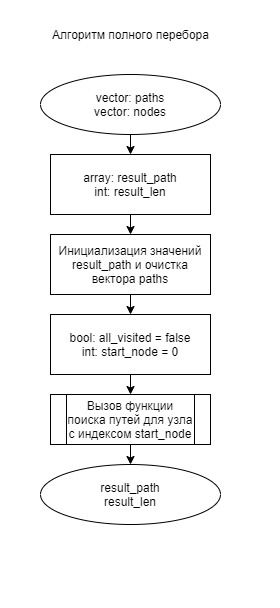
\includegraphics[scale=0.7]{brute_force_scheme_p_1}}
	\caption{Схема алгоритма полного перебора часть 1}
\end{figure}

\newpage

\begin{figure}[ph!]
	\center{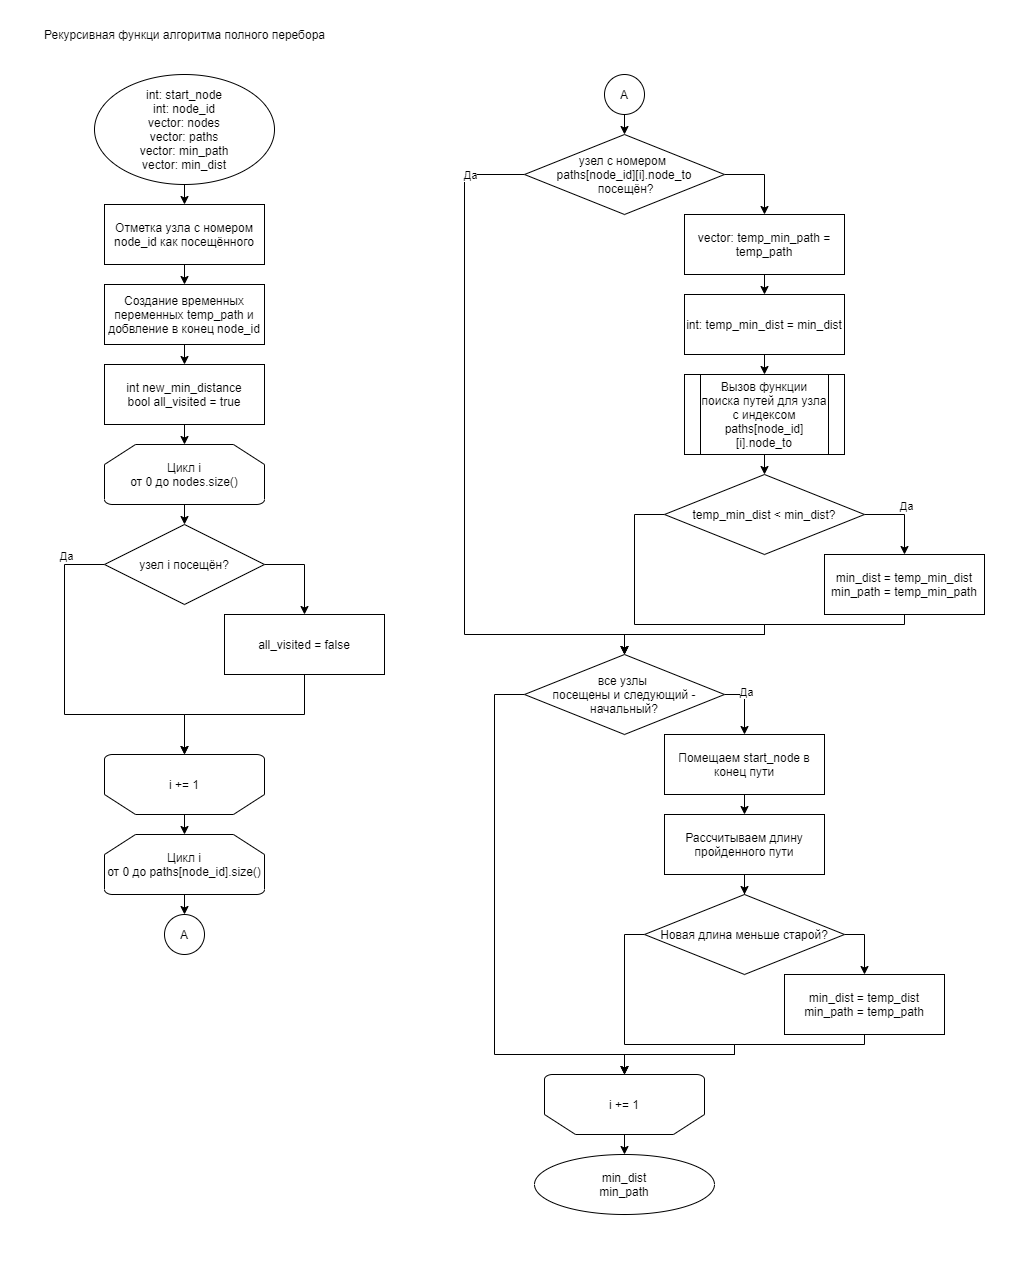
\includegraphics[scale=0.7]{brute_force_scheme_p_2}}
	\caption{Схема алгоритма полного перебора часть 2}
\end{figure}


\section{Муравьиный алгоритм}

Используемые типы и структуры данных включают в себя:
\begin{enumerate}
	\item integer, целое число - используется для хранения индексов массива, размера массива;
	\item vector, подвид списка - используется для хранения пути и узлов;
	\item bool, логическая переменная - используется в логических операциях;
	\item array, массив целых чисел - используется для хранения серии целых чисел.
\end{enumerate}

\begin{figure}[ph!]
	\center{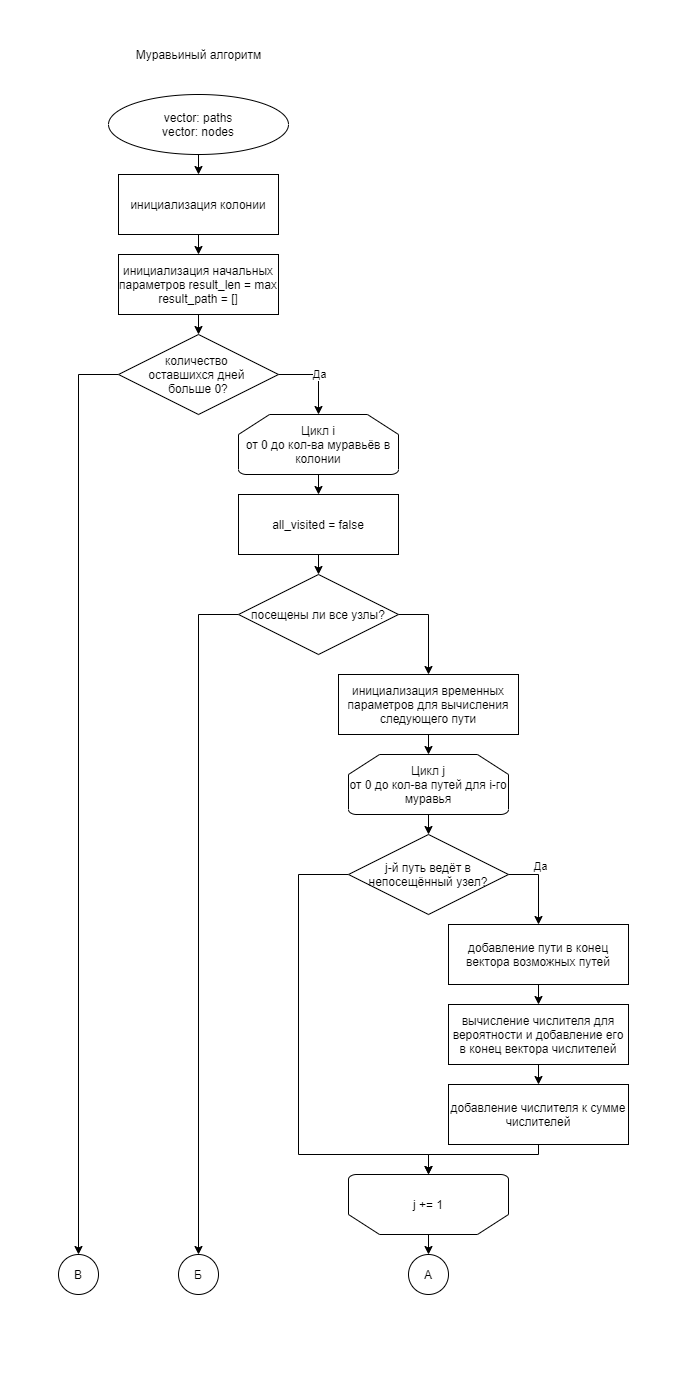
\includegraphics[scale=0.7]{ant_scheme_p_1}}
	\caption{Схема муравьиного алгоритма часть 1}
\end{figure}

\newpage

\begin{figure}[ph!]
	\center{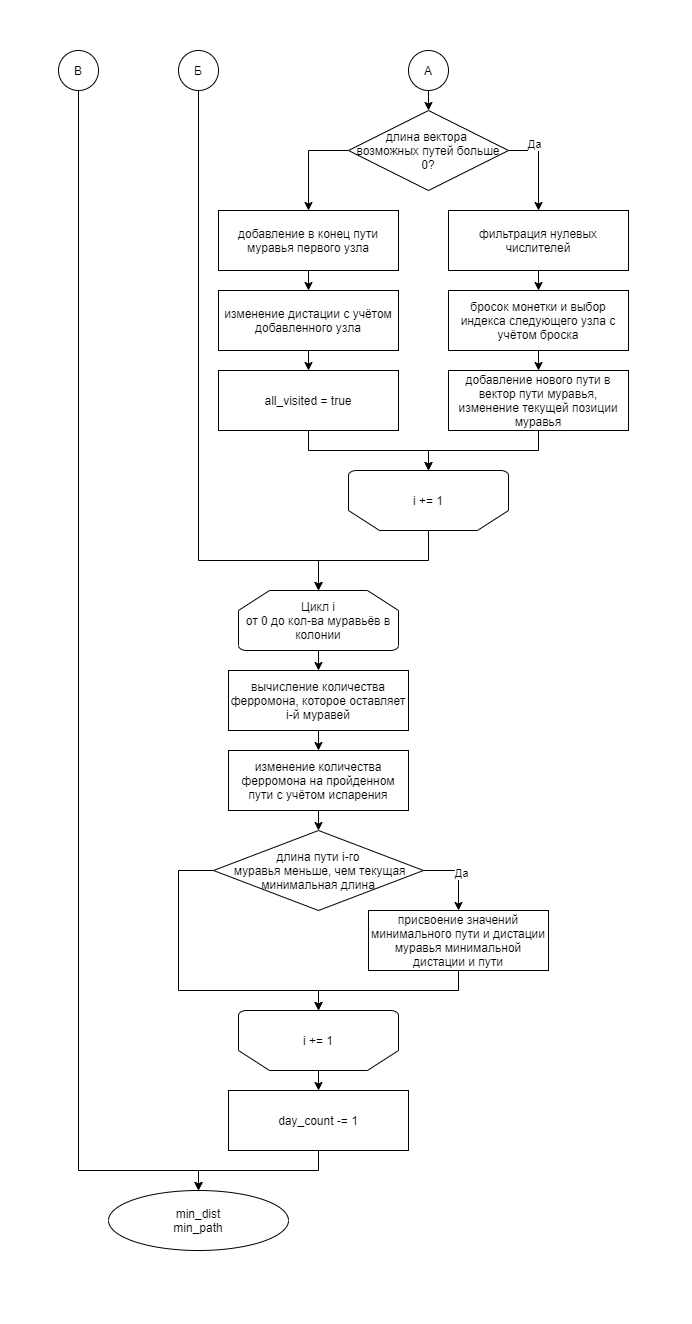
\includegraphics[scale=0.7]{ant_scheme_p_2}}
	\caption{Схема муравьиного алгоритма часть 2}
\end{figure}

\newpage

\section{Функциональная схема ПО}
На изображении ниже представлена функиональная схема разрабатываемого ПО. На вход подаётся вектор путей и вектор узлов, при помощи алгоритмов, реализованных на языке С++ мы получаем в результате работы наименьший путь и длину наименьшего пути.

\begin{figure}[ph!]
	\center{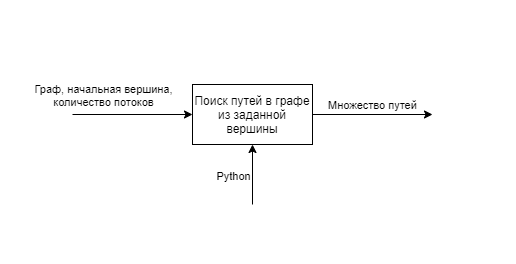
\includegraphics[scale=1.0]{func_scheme}}
	\caption{IDEF0 диаграмма разрабатываемой программы}
\end{figure}

\section{Вывод}
В данном разделе были рассмотрены схемы алгоритма полного перебора и муравьиного алгоритма. Были определены тесты для каждого алгоритма и описаны типы и структуры данных, использующихся в алгоритмах. Также была приведена функциональная схема разрабатываемого ПО.

\chapter{Технологический раздел}

В данном разделе будут рассмотрены подробности реализации описаных выше алгоритмов. Также будут обоснованы выбор языка программирования для реализации, выбор библиотек для проведения экспериментов и представлены важные фрагменты кода написанной в рамках работы программы.

\section{Выбор языка программирования}

В качестве языка программирования для реализации данной лабораторной работы использовался язык программирования C++ поскольку он предоставляет широкие возможности для эффективной реализации алгоритмов. В качестве среды разработки использовалась Microsoft Visual Studio 2019 по причине того, что данная среда имеет встроенные средства отладки и анализа работы программы, позволяющие быстро и эффективно писать код.

\section{Сведения о модулях программы}

Реализованное ПО состоит из трёх модулей:
\begin{enumerate}
	\item brute\_force - в данном модуле реализован алгоритм полного перебора;
	\item ants - в данном модуле реализован муравьиный алгоритм;
	\item lab\_6 - основной файл программы, где находится точка входа;
	\item tests - реализация тестов алгоритмов;
	\item time - реализация замеров времени работы программы.
\end{enumerate}

\section{Реализация алгоритмов}

\begin{lstlisting}[label=some-code-1,caption=Реализация алгоритма полного перебора]
void brute_force::brute_force_search(std::vector<std::vector<Path>>& path_matrix, std::vector<Node>& nodes, std::vector<int>& result_path, int& result_len)
{
	result_len = std::numeric_limits<int>::max();
	result_path.clear();
	bool all_visited = false;
	int start_node = 0;
	find_path_for_node(start_node, 0, nodes, path_matrix, result_path, result_len);
}

void brute_force::find_path_for_node(int &start_node, int node_id, std::vector<Node> nodes, std::vector<std::vector<Path>>& paths, std::vector<int>& min_path, int& min_dist)
{
	nodes[node_id].visited = true;
	
	std::vector<int> temp_path = min_path;
	temp_path.push_back(node_id);

	int new_min_distance;
	bool all_visited = true;
	for (auto& node : nodes)
	{
		if (node.visited == false)
			all_visited = false;
	}

	for (int i = 0; i < paths[node_id].size(); i++)
	{
		if (nodes[paths[node_id][i].node_to].visited == false)
		{
			std::vector<int> temp_min_path = temp_path;
			int temp_min_dist = min_dist;
			find_path_for_node(start_node, paths[node_id][i].node_to, nodes, paths, temp_min_path, temp_min_dist);
			if (temp_min_dist < min_dist)
			{
				min_dist = temp_min_dist;
				min_path = temp_min_path;
			}
		}

		if (nodes[paths[node_id][i].node_to].visited == true && all_visited && paths[node_id][i].node_to == start_node)
		{
			temp_path.push_back(start_node);

			int temp_dist = 0;
			int from;
			int to;

			for (int i = 0; i < temp_path.size() - 1; i++)
			{
				from = temp_path[i];
				to = temp_path[i + 1];
				for (auto& path : paths[from])
				{
					if (path.node_to == to)
						temp_dist += path.distance;
				}
			}

			if (temp_dist < min_dist)
			{
				min_dist = temp_dist;
				min_path = temp_path;
			}
		}
	}
}
\end{lstlisting}

\begin{lstlisting}[label=some-code-2,caption=Реализация муравьиного алгоритма]
void max_elem(std::vector<int> arr, int& max)
void ants::ant_search(std::vector<std::vector<Path>>& paths, std::vector<Node>& nodes, std::vector<int>& result_path, int& result_len)
{
	// initialize ants
	std::vector<ant> colony;

	for (int i = 0; i < ant_count; i++)
	{
		ant temp;
		temp.current_pos = rand() \% nodes.size();
		temp.distance = 0;
		temp.path.push_back(temp.current_pos);
		colony.push_back(temp);
	}

	result_len = std::numeric_limits<int>::max();
	result_path.clear();

	while (day_count > 0)
	{
		for (auto& ant : colony)
		{
			bool all_visited = false;
			while (!all_visited)
			{
				// Probability of going to node from paths
				double temp_sum = 0;
				std::vector<double> temp_top;
				std::vector<double> temp_prob;
				std::vector<Path> avalible_paths;

				for (auto& path : paths[ant.current_pos])
				{
					if (!ant.check_node_for_visided(path.node_to))
					{
						avalible_paths.push_back(path);
						double temp = pow(1.0f / (double)path.distance, alpha) * pow(path.ferromone, beta);
						temp_sum += temp;
						temp_top.push_back(temp);
					}
				}

				if (avalible_paths.size() > 0)
				{
					for (int i = 0; i < temp_top.size(); i++)
					{
						if (temp_top[i] > 0) 
							temp_prob.push_back(temp_top[i] / temp_sum);
					}

					double coin = ((double)rand() / (double)RAND_MAX);

					int index = 0;
					while (coin >= 0)
					{
						coin -= temp_prob[index];
						index++;
						if (index == avalible_paths.size())
							index = 0;
					}

					ant.path.push_back(avalible_paths[index].node_to);
					ant.current_pos = avalible_paths[index].node_to;
					ant.distance += avalible_paths[index].distance;
				}
				else
				{
					ant.path.push_back(ant.path[0]);

					for (int i = 0; i < paths[ant.current_pos].size(); i++)
					{
						if (paths[ant.current_pos][i].node_to == ant.path[0])
							ant.distance += paths[ant.current_pos][i].distance;
					}

					all_visited = true;
				}
			}
		}

		for (auto& ant_unit : colony)
		{
			double delta_ferr = ferr_for_ant / (double)ant_unit.distance;
			for (int i = 0; i < ant_unit.path.size() - 1; i++)
			{
				for (auto& path : paths[ant_unit.path[i]])
				{
					if (path.node_to == ant_unit.path[i + 1])
					{
						path.ferromone = (1 - evap_rate) * path.ferromone + delta_ferr;
					}
				}
			}

			if (ant_unit.distance < result_len)
			{
				result_len = ant_unit.distance;
				result_path = ant_unit.path;
			}

			ant_unit.reset_ant();
			ant_unit.current_pos = rand() \% nodes.size();
		}

		day_count -= 1;
	}
}
\end{lstlisting}

\section{Реализация тестирования алгоритмов}

Для тестирования алгоритмов было реализованы следующие тесты:
\begin{enumerate}
	\item тест на общем случае для алгоритма полного перебора  - на вход подаётся граф размерама n, возвращаемый результат сравнивается с заранее известным правильным результатом;
	\item тест на слишком маленьком графе - на вход подаётся граф с количеством вершин меньше двух, возвращаемый результат является расстоянием равным 0 и пустым путём;
	\item тест на неполносвязном  графе - на вход подаётся граф не являющийся полносвязным, возвращаемый результат является расстоянием равным 0 и пустым путём.
\end{enumerate}

\begin{lstlisting}[label=some-code-7,caption=Реализация тестов]      
#include "tests.h"

void test()
{
    brute_force br_fc;
    ants ants_s;

    std::vector<std::vector<Path>> path_mat = {
        {{7, 1, 1}, {8, 2, 1}, {7, 3, 1}, {3, 4, 1}},
        {{7, 0, 1}, {6, 2, 1}, {8, 3, 1}, {4, 4, 1}},
        {{8, 0, 1}, {6, 1, 1}, {4, 3, 1}, {7, 4, 1}},
        {{7, 0, 1}, {8, 1, 1}, {4, 2, 1}, {7, 4, 1}},
        {{3, 0, 1}, {4, 1, 1}, {7, 2, 1}, {7, 3, 1}}
    };

    std::vector<Node> nodes = {{1, 7, 0}, {4, 0, 0}, {9, 4, 0}, {8, 8, 0}, {2, 4, 0}};

    std::vector<int> result_path;
    int result_len = 0;

    // common data test for brute force
    br_fc.brute_force_search(path_mat, nodes, result_path, result_len);
    std::vector<int> true_result_path = { 0, 3, 2, 1, 4, 0 };
    int true_result_len = 24;
    std::cout << "Test on common data for brute force: ";
    if (true_result_len == result_len && result_path == true_result_path)
    {
        std::cout << "PASSED" << std::endl;
    }
    else
    {
        std::cout << "NOT PASSED" << std::endl;
    }

    // small graph data test for brute force

    path_mat.clear();
    nodes = { {1, 7, 0} };
    result_path.clear();
    result_len = 0;

    br_fc.brute_force_search(path_mat, nodes, result_path, result_len);

    true_result_len = 0;
    true_result_path.clear();

    std::cout << "Test on small graph data for brute force: ";
    if (true_result_len == result_len && result_path == true_result_path)
    {
        std::cout << "PASSED" << std::endl;
    }
    else
    {
        std::cout << "NOT PASSED" << std::endl;
    }

    // small graph data test for ants

    path_mat.clear();
    nodes = { {1, 7, 0} };
    result_path.clear();
    result_len = 0;

    ants_s.ant_search(path_mat, nodes, result_path, result_len);

    true_result_len = 0;
    true_result_path.clear();

    std::cout << "Test on small graph data for ant algorythm: ";
    if (true_result_len == result_len && result_path == true_result_path)
    {
        std::cout << "PASSED" << std::endl;
    }
    else
    {
        std::cout << "NOT PASSED" << std::endl;
    }

    // incorrect graph data test for brute force

    path_mat = {
        {{7, 1, 1}, {8, 2, 1}, {7, 3, 1}, {3, 4, 1}},
        {{7, 0, 1}, {6, 2, 1}, {8, 3, 1}, {4, 4, 1}},
        {{8, 0, 1}, {6, 1, 1}, {4, 3, 1}, {7, 4, 1}},
        {{7, 0, 1}, {8, 1, 1}, {4, 2, 1}, {7, 4, 1}},
        {{3, 0, 1}, {4, 1, 1}, {7, 2, 1}}
    };

    nodes = { {1, 7, 0}, {4, 0, 0}, {9, 4, 0}, {8, 8, 0}, {2, 4, 0} };

    result_path.clear();
    result_len = 0;

    br_fc.brute_force_search(path_mat, nodes, result_path, result_len);

    true_result_len = 0;
    true_result_path.clear();

    std::cout << "Test on incorrect graph data for brute force: ";
    if (true_result_len == result_len && result_path == true_result_path)
    {
        std::cout << "PASSED" << std::endl;
    }
    else
    {
        std::cout << "NOT PASSED" << std::endl;
    }

    // incorrect graph data test for ants

    path_mat = {
        {{7, 1, 1}, {8, 2, 1}, {7, 3, 1}, {3, 4, 1}},
        {{7, 0, 1}, {6, 2, 1}, {8, 3, 1}, {4, 4, 1}},
        {{8, 0, 1}, {6, 1, 1}, {4, 3, 1}, {7, 4, 1}},
        {{7, 0, 1}, {8, 1, 1}, {4, 2, 1}, {7, 4, 1}},
        {{3, 0, 1}, {4, 1, 1}, {7, 2, 1}}
    };

    nodes = { {1, 7, 0}, {4, 0, 0}, {9, 4, 0}, {8, 8, 0}, {2, 4, 0} };

    result_path.clear();
    result_len = 0;

    ants_s.ant_search(path_mat, nodes, result_path, result_len);

    true_result_len = 0;
    true_result_path.clear();

    std::cout << "Test on incorrect graph data for ant algorythm: ";
    if (true_result_len == result_len && result_path == true_result_path)
    {
        std::cout << "PASSED" << std::endl;
    }
    else
    {
        std::cout << "NOT PASSED" << std::endl;
    }
}
\end{lstlisting}

\section{Вывод}
В данной разделе были представлены реализации алгоритма полного перебора и муравьиного алгоритма, а также представлена реализация модуля тестирования реализованных алгоритмов.

\chapter{Экспериментальный раздел}

В данном разделе описывается подбор параметров муравьиного алгоритма и измерентя временных характеристики алгоритмов полного перебра и муравьиного алгоритма, а также делается вывод об эффективности алгоритмов.

\section{Технические характеристики}
\begin{itemize}
	\item Операционная система - Windows 10, 64-bit;
	\item Оперативная память - 16 GiB;
	\item Процессор - Intel(R) Core(TM) i7-9750H CPU @ 2.60GHz 2.59 GHz, 6 ядер, 12 потоков.
\end{itemize}

\section{Результаты подбора параметров}

В муравьином алгоритме вычисления производятся на основе нескольких настроиваих параметров. По причине этого нам необходимо подобрать лучшую комбинацию параметров, при которой алгоритм работает быстрее и лучше. Эксперимент проводится на графе имеющем 10 узлов с расстояниями от 1 до 10. Такой размер выбран по причине того, что 10 узлов могут быть обработаны алгоритмом полного перебора за приемлемый отрезок времени. Параметры перебора: количество муравьёв - 5, количество дней - от 50 до 500 с шагом 50, количество ферромона, которое переносит один муравей - от 10 до 50 с шагом 10, альфа - от 0 до 1 с шагом 0.2, уровень испарения ферромонов от 0 до 1 с шагом 0.2. Так как количество вариаций превышает несколько тысяч, в таблицы добавлялись только результаты с путём, 80\% которого меньше идеального пути, полученного с помощью алгоритмов полного перебора.\\

\noindent Обозначения: \\
iters - кол-во итераций.\\
ants - кол-во муравьёв.\\
f - кол-во ферромона для одного муравья.\\
min - минимальная дистанция для данного набора параметров.\\
true min - истинная минимальная дистанция, найденная полным перебором.\\

\begin{table}[ph!]
  \begin{center}
    \captionsetup{justification=raggedright}
     \caption{Перебор параметров часть 1}
    \label{tab:workcost_classic}
    \begin{tabular}{c|c|c|c|c|c|c|c}
      \textbf{iters} & \textbf{ants}  & \textbf{$\alpha$}  & \textbf{$\beta$} & \textbf{$p$} & \textbf{f}  & \textbf{min}  & \textbf{true min}\\
      \hline	
	150 & 5 & 0 & 1 & 0 & 10 & 34.6 & 28\\
	150 & 5 & 0 & 1 & 0.2 & 40 & 33.8 & 28\\
	200 & 5 & 0.4 & 0.6 & 0.4 & 20 & 34.8 & 28\\
	250 & 5 & 0 & 1 & 0.4 & 40 & 34.2 & 28\\
	250 & 5 & 0 & 1 & 0.8 & 10 & 34.8 & 28\\
	250 & 5 & 0 & 1 & 0.8 & 40 & 33.8 & 28\\
	250 & 5 & 0.2 & 0.8 & 0.8 & 20 & 34.6 & 28\\
	300 & 5 & 0 & 1 & 0 & 10 & 34 & 28\\
	300 & 5 & 0 & 1 & 0.2 & 10 & 34.6 & 28\\
	300 & 5 & 0 & 1 & 0.4 & 10 & 33.8 & 28\\
	300 & 5 & 0 & 1 & 0.6 & 10 & 34.8 & 28\\
	300 & 5 & 0.4 & 0.6 & 0.4 & 10 & 34.8 & 28\\
	300 & 5 & 0.6 & 0.4 & 0.6 & 40 & 34.4 & 28\\
	300 & 5 & 0.6 & 0.4 & 0.8 & 10 & 33.6 & 28\\
    \end{tabular}
  \end{center}
\end{table}


\begin{table}[ph!]
  \begin{center}
    \captionsetup{justification=raggedright}
     \caption{Перебор параметров часть 2}
    \label{tab:workcost_classic}
    \begin{tabular}{c|c|c|c|c|c|c|c}
      \textbf{iters} & \textbf{ants}  & \textbf{$\alpha$}  & \textbf{$\beta$} & \textbf{$p$} & \textbf{f}  & \textbf{min}  & \textbf{true min}\\
      \hline	
	350 & 5 & 0 & 1 & 0 & 20 & 34.4 & 28\\
	350 & 5 & 0 & 1 & 0 & 30 & 33.8 & 28\\
	350 & 5 & 0 & 1 & 0.8 & 10 & 33.8 & 28\\
	350 & 5 & 0 & 1 & 0.8 & 30 & 34.8 & 28\\
	350 & 5 & 0.2 & 0.8 & 0.2 & 20 & 34.8 & 28\\
	350 & 5 & 0.2 & 0.8 & 0.4 & 20 & 34.8 & 28\\
	350 & 5 & 0.2 & 0.8 & 0.8 & 40 & 34.8 & 28\\
	350 & 5 & 0.4 & 0.6 & 0.8 & 20 & 34.8 & 28\\
	350 & 5 & 0.6 & 0.4 & 0 & 30 & 34.6 & 28\\
	400 & 5 & 0 & 1 & 0 & 20 & 34.6 & 28\\
	400 & 5 & 0 & 1 & 0 & 30 & 34.6 & 28\\
	400 & 5 & 0 & 1 & 0.4 & 20 & 34.2 & 28\\
	400 & 5 & 0 & 1 & 0.8 & 20 & 34.8 & 28\\
	400 & 5 & 0 & 1 & 0.8 & 30 & 34.4 & 28\\
	400 & 5 & 0.2 & 0.8 & 0 & 30 & 34.2 & 28\\
	400 & 5 & 0.2 & 0.8 & 0.6 & 30 & 34.8 & 28\\
	400 & 5 & 0.2 & 0.8 & 0.6 & 40 & 34 & 28\\
	400 & 5 & 0.2 & 0.8 & 0.8 & 30 & 34.4 & 28\\
	400 & 5 & 0.4 & 0.6 & 0.4 & 10 & 34.8 & 28\\
	400 & 5 & 0.4 & 0.6 & 0.6 & 10 & 34.4 & 28\\
	400 & 5 & 0.6 & 0.4 & 0 & 10 & 34.8 & 28\\
    \end{tabular}
  \end{center}
\end{table}

\begin{table}[ph!]
  \begin{center}
    \captionsetup{justification=raggedright}
     \caption{Перебор параметров часть 3}
    \label{tab:workcost_classic}
    \begin{tabular}{c|c|c|c|c|c|c|c}
      \textbf{iters} & \textbf{ants}  & \textbf{$\alpha$}  & \textbf{$\beta$} & \textbf{$p$} & \textbf{f}  & \textbf{min}  & \textbf{true min}\\
      \hline	
	450 & 5 & 0 & 1 & 0 & 30 & 34.6 & 28\\
	450 & 5 & 0 & 1 & 0.2 & 10 & 34.4 & 28\\
	450 & 5 & 0 & 1 & 0.4 & 20 & 34.4 & 28\\
	450 & 5 & 0 & 1 & 0.4 & 30 & 34 & 28\\
	450 & 5 & 0 & 1 & 0.4 & 40 & 34.6 & 28\\
	450 & 5 & 0 & 1 & 0.8 & 10 & 34.4 & 28\\
	450 & 5 & 0 & 1 & 0.8 & 20 & 34.2 & 28\\
	450 & 5 & 0.2 & 0.8 & 0.6 & 10 & 34 & 28\\
	450 & 5 & 0.2 & 0.8 & 0.6 & 40 & 34.8 & 28\\
	450 & 5 & 0.4 & 0.6 & 0 & 20 & 34.8 & 28\\
	450 & 5 & 0.4 & 0.6 & 0.8 & 30 & 34.2 & 28\\
	450 & 5 & 0.6 & 0.4 & 0 & 20 & 34.6 & 28\\
	450 & 5 & 0.6 & 0.4 & 0.4 & 10 & 34.8 & 28\\
	450 & 5 & 0.8 & 0.2 & 0.2 & 30 & 34.8 & 28\\
	450 & 5 & 0.8 & 0.2 & 0.4 & 10 & 34.8 & 28\\
	500 & 5 & 0 & 1 & 0 & 30 & 34.2 & 28\\
	500 & 5 & 0 & 1 & 0.4 & 40 & 34.8 & 28\\
	500 & 5 & 0 & 1 & 0.6 & 20 & 34.4 & 28\\
	500 & 5 & 0 & 1 & 0.6 & 30 & 34.8 & 28\\
	500 & 5 & 0 & 1 & 0.8 & 10 & 34.8 & 28\\
	500 & 5 & 0 & 1 & 0.8 & 30 & 34.4 & 28\\
	500 & 5 & 0 & 1 & 0.8 & 40 & 34.4 & 28\\
	500 & 5 & 0.2 & 0.8 & 0.2 & 10 & 34.6 & 28\\
	500 & 5 & 0.2 & 0.8 & 0.4 & 40 & 34.6 & 28\\
	500 & 5 & 0.2 & 0.8 & 0.8 & 20 & 34.8 & 28\\
	500 & 5 & 0.2 & 0.8 & 0.8 & 30 & 34 & 28\\
	500 & 5 & 0.4 & 0.6 & 0.6 & 40 & 34.6 & 28\\
	500 & 5 & 0.4 & 0.6 & 0.8 & 10 & 34.2 & 28\\
	500 & 5 & 0.6 & 0.4 & 0.4 & 30 & 34.8 & 28\\
	500 & 5 & 0.6 & 0.4 & 0.6 & 40 & 33.8 & 28\\
    \end{tabular}
  \end{center}
\end{table}

\noindent Набор параметров, который позволил найти наилучший путь:\\
количество итераций - 300;\\
количество муравьёв - 5;\\ 
альфа - 0.6;\\
бета - 0.4;\\
уровень испарения - 0.8;\\
количество ферромона для муравья - 10.\\

\newpage

\section{Результаты экспериментов}

\begin{table}[ph!]
  \begin{center}
    \captionsetup{justification=raggedright}
     \caption{Время работы алгоритмов}
    \label{tab:workcost_classic}
    \begin{tabular}{c|c|c}
      \textbf{кол-во узлов} & \textbf{t полного перебора (нс)}  & \textbf{t муравьиного алгоритма (нс)}\\
      \hline	
		2 & 41140 & 50990360\\
		3 & 95460 & 123472630\\
		4 & 209590 & 128274640\\
		5 & 692210 & 137194230\\
		6 & 4723110 & 312229910\\
		7 & 41685220 & 458251240\\
		8 & 212235570 & 418253070\\
		9 & 1672092450 & 495543340\\
		10 & 14021435680 & 509634800\\
    \end{tabular}
  \end{center}
\end{table}

\begin{figure}[ph!]
	\center{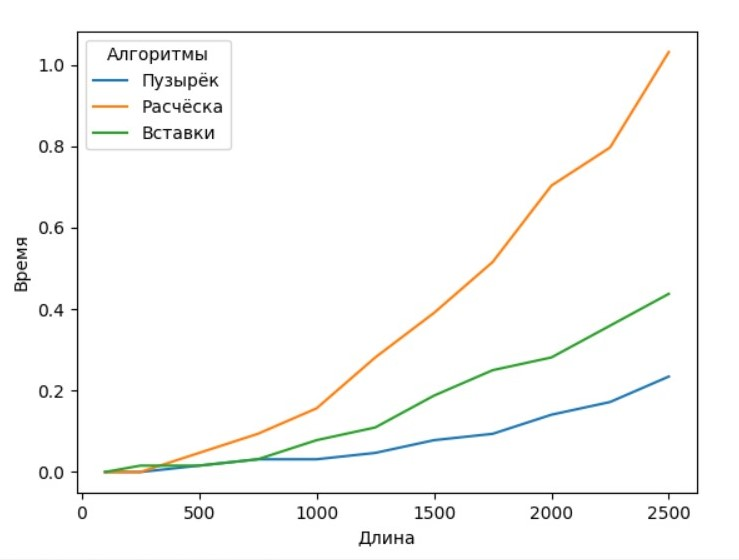
\includegraphics[scale=0.7]{res_graph}}
	\caption{График зависимости времени работы от размерности массивов}
\end{figure}

\section{Вывод}
В результате эксперимента было получено, что оптимальными параметрами для муравьиного алгоритма являются количество итераций - 300, количество муравьёв - 5, альфа - 0.6, бета - 0.4, уровень испарения - 0.8, количество ферромона для муравья - 10. При сравнении времени выполнения при достижении 10 узлов муравьиный алгоритм работает более чем в 27 раз быстрее. В результате можно сделать вывод о том, что использование муравьиного алгоритма позволяет решать задачу коммивояжера значительно быстрее, чем алгоритм полного перебора.